\qrchapter{https://forgottenpillar.com/rsc/sw-fp-chapter14}{Waanzilishi wa Kiadventista na fundisho la Utatu}

Dada White aliandika kwamba waanzilishi wa awali wa Waadventista \egwinline{wanapaswa kutoa ushuhuda wao kuhusu yanayojumuisha ukweli kwa wakati huu}[Lt329-1905.18; 1905][https://egwwritings.org/read?panels=p8455.24] kwa sababu \egwinline{wamejifunza kuepuka makosa na hatari, na je, hawana uwezo wa kutoa nasaha zenye hekima}[7T 287.3; 1902][https://egwwritings.org/read?panels=p117.1637]? Katika maandishi yao, tunaona maoni yao ya upamoja kuhusu \emcap{Umbile la Mungu}, na kwamba wameepuka hitilafu ya Utatu. Kuna mengi ya kuandika kuhusu mada hii kwa sababu waanzilishi wa Kiadventista waliacha maandiko mengi yanayohusika moja kwa moja au kwa njia isiyo ya moja kwa moja na fundisho la Utatu. Lakini tutaangalia baadhi ya shuhuda kutoka kwa James White na kaka Loughborough kwa sababu tumesoma baadhi ya makala zao kuhusu \emcap{Umbile la Mungu}. Pia, tutalinganisha ushuhuda wao kwa Roho ya Unabii kama tulivyofanya hadi tulipofikia.

James White, katika Review and Herald, aliorodhesha \others{baadhi ya \textbf{hekaya maarufu} za enzi hizo}”, akisema: “\others{Hapa tunaweza kutaja \textbf{Utatu, ambao \underline{huondoa Umbile la Mungu, na wa Mwana wake Yesu Kristo,} }na kunyunyiza au kumwagiwa badala ya ‘kuzikwa pamoja na Kristo katika ubatizo,’ ‘kupandwa katika mfano wa mauti yake:’ lakini tunapita kutoka kwa \textbf{hadithi hizi }hadi kuona moja ambayo inachukuliwa kuwa wa kitakatifu na karibu wote wanaodai kuwa Wakristo, Wakatoliki na pia Kiprotestanti. Ni, mabadiliko ya Sabato ya amri ya nne kutoka siku ya saba hadi siku ya kwanza ya juma.}[James S. White, Review \& Herald, December 11, 1855, p. 85.15][http://documents.adventistarchives.org/Periodicals/RH/RH18551211-V07-11.pdf]

James White anamaanisha nini anaposema kwamba Utatu \others{huondoa Umbile la Mungu, na wa Mwana wake Yesu Kristo}? Katika Day Star, aliandika:

\others{…kundi fulani ambalo \textbf{linamkana Bwana Mungu pekee na Bwana wetu Yesu Kristo}. Kundi hili haliwezi kuwa lingine zaidi ya wale ambao \textbf{hufanya kuwa ya kiroho uwepo wa Baba na Mwana}, \textbf{kama \underline{Nafsi mbili tofauti}, \underline{halisi}, \underline{zinazoonekana}}, pia mji halisi wa Mungu na kiti cha enzi cha Daudi... Njia ambayo wanaofanya mambo kuwa ya kiroho wamefanya kuondoa au \textbf{kumkana Bwana Mungu pekee na Bwana wetu Yesu Kristo ni kwanza kutumia \underline{kanuni ya zamani ya utatu isiyo ya kimaandiko}}, yaani, kwamba Yesu Kristo ni Mungu wa milele, ingawa hawana kifungu hata kimoja cha kuunga mkono, wakati tuna ushuhuda wa maandiko wazi kwa wingi \textbf{kwamba Yeye ni Mwana wa Mungu wa milele.}}[James White, Day Star, Jan 24, 1846][https://m.egwwritings.org/en/book/741.25\#27]

Kuondoa Umbile la Mungu na Mwana wake kunafanyika kwa kuwakana Wao kama Nafsi mbili tofauti, halisi, na zinazoonekana. Fundisho juu ya Umbile la Mungu linafundisha kwamba Baba ana nafsi halisi, \textit{inayoonekana}.

Katika makala ya Adventist Review and Sabbath Herald kutoka Aprili 4, 1854, James White aliorodhesha hoja 10 za \textit{sababu za Kikatoliki za kutunza Jumapili}”, ambapo alisema kwamba Jumapili \others{ni siku iliyotengwa na mitume kwa \textbf{heshima ya Utatu Aliye Mtakatifu zaidi}}[The Advent Review, and Sabbath Herald, vol. 5 April 4, 1854, p. 86][https://egwwritings.org/read?panels=p1643.2867]. Hapa tunaona pia maelewano kati ya J. B. Frisbie na James White kwa maoni yao kwamba Sabato imewekwa wakfu kwa Mungu wa kibiblia Aliyeonyeshwa katika hoja ya kwanza ya \emcap{Kanuni za Msingi}, na Jumapili ni wakfu kwa Mungu wa utatu. Tatizo kuu la fundisho la Utatu ni kwamba \others{huondoa Umbile la Mungu, na wa Mwanawe Yesu Kristo}. Katika Life Incidents, aliandika zaidi kuhusu kwa nini hii ni hivyo.

\others{\textbf{Yesu alisali kwamba wanafunzi wake wawe kitu kimoja kama alivyokuwa \underline{mmoja na Baba yake}}. \textbf{Maombi haya hayakuwaza mfuasi mmoja mwenye vichwa kumi na viwili, bali wanafunzi kumi na wawili, waliofanywa moja kwa lengo na juhudi katika njia ya Bwana wao}. \textbf{\underline{Wala Baba na Mwana si sehemu za ‘Mungu watatu-mmoja.}}’\footnote{Nukuu hiyo hiyo inapatikana katika kitabu cha James White “\textit{The Law and the Gospel}” na tofauti moja. Anasema, “\textit{Wala Baba na Mwana si sehemu za \underline{huluki moja}}”; katika “\textit{Life Incidents}”, aliandika “sehemu za ‘\underline{Mungu watatu-mmoja}’“. Tazama \href{https://egwwritings.org/?ref=en_LAGO.1.2&para=1492.10}{James S. White, The Law and the Gospel p. 1.2}.} \textbf{\underline{Wao ni Nafsi mbili tofauti}}, \textbf{lakini mmoja katika muundo na utimilifu wa ukombozi}. Waliokombolewa, kutoka kwa wa kwanza ambaye anashiriki katika ukombozi mkuu, hadi wa mwisho, wote wanapeana heshima, na utukufu, na sifa, za wokovu wao kwa \textbf{Mungu na Mwanakondoo pia}.}[James S. White, Life Incidents, p.343.2][https://egwwritings.org/read?panels=p1462.1743]

Dada White aliandika vile vile kuhusu sala ya Kristo:

\egw{Mzigo wa maombi hayo ulikuwa kwamba wanafunzi Wake wawe \textbf{kitu kimoja kama vile Yeye alivyokuwa Mmoja na Baba}; umoja uliokaribi-ana hivi kwamba, \textbf{ingawa walikuwa \underline{Nafsi wawili tofauti}}, kulikuwa na \textbf{umoja kamili ya roho, kusudi, na vitendo}. Nia ya Baba ilikuwa nia ya Mwana.}[Lt1-1882.1; 1882][https://egwwritings.org/read?panels=p4120.5]

\egw{\textbf{Umoja uliopo kati ya Kristo na wanafunzi wake \underline{hauharibu ubinafsi wa kila mmoja}}. Wao ni wamoja kwa kusudi, akilini, katika tabia, \textbf{lakini \underline{sio kibinafsi}}. \textbf{Ni hivyo kwamba Mungu na Kristo ni mmoja}.}[MH, 421 422; 1905][https://egwwritings.org/read?panels=p135.2177]

Baba na Mwana hawajumuishi nafsi mmoja wala huluki moja. Baba na Mwana ni mmoja, kama vile Kristo na wanafunzi Wake ni wamoja—wamoja katika roho, kusudi, akili, na tabia.

Wataalamu wengi wa utatu wa Waadventista wanamtoza James White na waanzilishi wengine wa mapema uariani au nusu-ariani, wakidai kwamba walimfanya Kristo kuwa duni kwa Baba. Hii si kweli. Hebu tusome ushuhuda wa James White juu ya jambo hili.

\others{Paulo anathibitisha juu ya \textbf{Mwana wa Mungu kwamba alikuwa katika namna ya Mungu}, na kwamba \textbf{\underline{alikuwa sawa na Mungu}}. ‘\textbf{Ambaye kwa kuwa yu namna ya Mungu hakuona kuwa sawa na Mungu kuwa ni kitu cha kushikamana nacho}.’ Fil. 2:6. Sababu isio wizi kwa Mwana \textbf{kuwa sawa na Baba ni ukweli kwamba yeye ni sawa}.  Ikiwa Mwana si sawa na Baba, basi ni wizi kwake kuwa na cheo mwenyewe pamoja na Baba.}

\othersnogap{\textbf{\underline{Utatu usioelezeka unaofanya miungu mitatu katika moja na moja katika tatu, ni mbaya kutosha}}; \textbf{lakini imani hiyo ya Unitariani inayomfanya Kristo kuwa duni kwa Baba ni mbaya zaidi}. Je! Mungu alimwambia aliye duni, Na tumfanye mwanadamu kwa mfano wetu?’}[James S. White, The Advent Review and Sabbath Herald, November 29, 1877, p. 171][https://documents.adventistarchives.org/Periodicals/RH/RH18771129-V50-22.pdf]

Tatizo la wataalamu wa utatu wa Kiadventista liko kwa kuwa wao wenyewe hawawezi kueleza kikamilifu uungu wa Kristo zaidi ya kupitia dhana ya Utatu. Waadventista waanzilishi waliamini katika uungu kamili wa Kristo lakini walikataa Utatu kwa sababu unaharibu \emcap{ubinafsi wa Mungu}. \others{Utatu usioelezeka unaofanya miungu mitatu katika moja na moja katika tatu, \textbf{ni mbaya kutosha}}. Chini ni taarifa nyingine kutoka kwa James White ambapo yeye alilinganisha Imani ya Waadventista Wasabato na imani ya Wabaptisti wa Sabato. Waadventista Wasabato hawakuamini Utatu tofauti na Wabaptisti wa Siku ya Saba. James White alisema kuwa, kuhusu uungu wa Kristo, Waadventista Wasabato wanashikilia karibu sana na utatu Wabaptisti wa siku ya saba ambao hawashikilii kesi yoyote kule.

\others{\textbf{Tofauti kuu kati ya miili miwili ni swali la kutokufa}. \textbf{Shirika la S.D. Waadventista wanashikilia uungu wa Kristo karibu sana na utatu, kwamba tunaufahamu hakuna kesi hapa}. Na kama matumizi ya vitendo kwenye somo la Karama za Roho kwetu watu na kwa kazi yetu inaeleweka vyema na ndugu zetu wa S. D. Baptist, wanadhihirisha kujali kwa kiasi kwa sababu hii.}[James S. White, The Advent Review and Sabbath Herald, October 12, 1876, p. 116][https://documents.adventistarchives.org/Periodicals/RH/RH18761012-V48-15.pdf]

Ushahidi huu unapaswa kuibua maswali kwa kila mwataalamu wa utatu wa Kiadventista. Inawezaje kuwa kwamba waanzilishi wa Kiadventista walishikamana na uungu wa Kristo kama waamini wa utatu walivyofanya, lakini wakakataa fundisho la Utatu? Ni kwa njia gani Kristo alikuwa Mungu kikamilifu, ikiwa hakuwa sehemu ya Mungu aliyeunganishwa watatu katika mmoja? Jibu ni rahisi na la Kibiblia kabisa. Kristo ni Mungu kwa ukamilifu, kama Baba yake, kwa sababu alizaliwa kwa sura ya wazi ya nafsi ya Baba; hivyo, Alirithi asili kamili ya kimungu kutoka kwa Baba Yake.

\egw{Sadaka kamili imetolewa; kwa maana ‘Mungu aliupenda ulimwengu, hata akatoa Mwana mzaliwa wa pekee,’—\textbf{si mwana kwa kuumbwa}, kama walivyokuwa malaika, wala mwana kwa kufanywa wana, kama vile mwenye dhambi aliyesamehewa, lakini \textbf{Mwana \underline{aliyezaliwa} kwa sura ya wazi ya nafsi ya Baba}, na katika mng'ao wote wa enzi na utukufu wake, \textbf{aliye sawa na Mungu} katika mamlaka, adhama, na \textbf{ukamilifu wa kimungu}. \textbf{Ndani yake unakaa utimilifu wote wa Uungu, kwa jinsi ya kimwili}.}[ST May 30, 1895, par. 3; 1895][https://egwwritings.org/read?panels=p820.12891]

Uungu kamili wa Kristo hautegemei juu ya \emcap{ubinafsi} uliounganishwa wa Mungu, bali juu ya Uwana wake na Baba. Biblia haimrejelei kamwe Kristo kwa neno “Mungu mmoja”—Baba pekee anarejelewa kwa neno “Mungu mmoja”\footnote{Yohana 17:3; 1. Wakorintho 8:6; 1. Timotheo 2:5; Waefeso 4:6} \footnote{Tunasoma uungu kamili wa Kristo kwa kina katika kitabu cha pili cha Mradi wa Nguzo Iliyosahaulika - “Kugundua upya Nguzo”}. Yesu, Mwana wa Mungu, ni Mungu kamili lakini haielezwi kuwa \others{\textbf{Mungu mmoja}, \textbf{huluki wa kibinafsi, wa kiroho}} katika hoja ya kwanza ya \emcap{Kanuni za Msingi}.

\egw{Bwana Yesu Kristo, Mwana pekee wa Baba, \textbf{kweli ni Mungu katika ukomo, \underline{lakini sivyo katika ubinafsi}}.}[Ms116-1905.19; 1905][https://egwwritings.org/read?panels=p10633.25]

Ndugu J. N. Loughborough aliombwa kujibu swali, \others{Ni upinzani gani zito uko kwenye fundisho la Utatu?}[Swali liliulizwa na Ndugu W. W. Giles na lilipelekwa kwa James S. White, ambaye alipeleka swali hilo kwa Ndugu John N. Loughborough.]. Tunaposoma jibu lake, acheni tujaribu kuelewa baadhi ya sababu kwa nini waanzilishi wa awali hawakushikamana na fundisho hili.

\others{Kuna pingamizi nyingi ambazo tunaweza kuhimiza, lakini kwa sababu ya nafasi yetu ndogo sisi tutapunguza hadi tatu zifuatazo: \textbf{1. Ni kinyume na akili timamu. 2. Ni kinyume na maandiko. 3. Asili yake ni ya Kipagani na ya ajabu.}}

\othersnogap{Nafasi hizi tutazieleza kwa ufupi kwa mpangilio wao. Na 1. \textbf{Haina uthabiti na akili timamu kuongelea watatu kuwa Mmoja, na mmoja kuwa watatu}. \textbf{Au kama wengine kulieleza, akimwita Mungu ‘Mungu wa Utatu,’ au ‘Mungu watatu-mmoja.’} \textbf{Ikiwa Baba, Mwana, na Roho Mtakatifu ni kila Mungu, ingekuwa ni Miungu watatu; maana mara tatu mtu si mmoja, lakini tatu}. \textbf{\underline{Kuna hali ambayo wao ni mmoja, lakini sio mtu mmoja, kama inavyodaiwa na Waamini Utatu}}}.

\othersnogap{2. \textbf{Ni kinyume na Maandiko}. \textbf{Karibu sehemu yoyote ya Agano Jipya tunaweza kufungua ambayo ina nafasi ya kusema juu ya Baba na Mwana, inawawakilisha kama nafsi mbili tofauti}. \textbf{\underline{Sura ya kumi na saba ya Yohana pekee inatosha kukanusha fundisho la Utatu}}. \textbf{Zaidi ya mara arobaini katika sura hiyo moja Kristo anazungumza juu ya Baba yake kama nafsi tofauti na yeye mwenyewe}. Baba yake alikuwa mbinguni na yeye alikuwa duniani. Baba alikuwa amemtuma. Amepewa wale walioamini. Alikuwa basi aende kwa Baba.\textbf{ Na katika ushuhuda huu anaotuonyesha katika kile kinachojumuisha umoja wa Baba na Mwana}.\textbf{\underline{ Ni sawa na umoja wa washiriki wa kanisa la Kristo}}. ‘\textbf{Ili \underline{wote} wawe moja; \underline{kama} wewe, Baba, ulivyo ndani yangu, nami ndani yako, \underline{hao nao} wawe moja ndani yetu}; kwamba ulimwengu upate kusadiki kwamba ndiwe uliyenituma. Na \textbf{utukufu ulionipa nao nawapea}; ili \textbf{wawe kitu kimoja}, \textbf{kama sisi tulivyo umoja.}’ \textbf{Wa moyo mmoja na nia moja}. \textbf{Ya kusudi moja} katika mpango wote uliopangwa kwa ajili ya wokovu wa mwanadamu. \textbf{\underline{Soma sura ya kumi na saba ya Yohana, na uone ikiwa haivunji kabisa fundisho la Utatu}}.}

\othersnogap{\textbf{Ili kuamini fundisho hilo, tunaposoma maandiko ni lazima tuamini kwamba Mungu alijituma mwenyewe katika ulimwengu, alikufa ili kuupatanisha ulimwengu na nafsi yake, alijiinua kutoka kwa aliyekufa, akapaa kwake mbinguni, anasihi mbele zake mbinguni ili kupatanisha ulimwengu kwake mwenyewe, na ndiye mpatanishi pekee kati ya mtu na yeye mwenyewe}. Haitafanya kuchukua nafasi ya asili ya kibinadamu ya Kristo (kulingana na waamini Utatu) kama Mpatanishi; kwani Clarke anasema, ‘Damu ya mwanadamu haiwezi kumpendeza Mungu kuliko damu ya nguruwe.’ Fafanua 2 Samweli 21:10. \textbf{Tunapaswa kuamini pia kwamba katika bustani Mungu alijiomba mwenyewe, ikiwa  ikiwezekana, kukiacha kikombe kipite kutoka kwake mwenyewe, na \underline{upuuzi kama hizo} elfu na elfu}.}

\othersnogap{\textbf{Soma kwa makini maandiko yafuatayo, ukiyalinganisha na wazo kwamba Kristo ndiye Mungu Mwenye Nguvu Zote, Aliyepo Pote, Aliye Juu Zaidi, na pekee anayeishi mwenyewe: Yohana 14:28; 17:3; 3:16; 5:19, 26; 11:15; 20:19; 8:50; 6:38; Marko 13:32; Luka 6:12; 22:69; 24:29; Mathayo 3:17; 27:46; Wagalatia 3:20; 1 Yohana 2:1; Ufunuo 5:7; Matendo 17:31. Pia tazama Mathayo 11:25, 27; Luka 1:32; 22:42; Yohana 3:35, 36; 5:19, 21, 22, 23, 25, 26; 6:40; 8:35, 36; 14:13; 1 Wakorintho 15:28, nk}.}

\othersnogap{\textbf{Neno Utatu halipatikani popote katika Maandiko}. \textbf{Nakala kuu inayopaswa kufundisha ni 1 Yohana 5:7\footnote{J. N. Loughborough alifanya makosa ya uchapishaji katika hati asili, alitaka kuonyesha 1 Yohana 5:7}, ambayo ni tafsiri}. Clarke anasema, ‘\textbf{Kati ya mia moja na kumi na tatu, maandishi hayapo katika mia moja na kumi na mbili. haitokei katika muswada wowote kabla ya karne ya kumi. Na mahali pa kwanza maandishi yanapatikana katika Kigiriki, ni katika Tafsiri ya Kigiriki ya matendo ya Mtaguso wa Laterani, uliofanyika A. D. 1215}.’ - Maoni. juu Yohana 1, na maelezo mwishoni mwa sura.}

\othersnogap{3. \textbf{Asili yake ni ya Kipagani na ya ajabu}. Badala ya kutuelekeza kwenye maandiko kwa uthibitisho wa utatu, tunaelekezwa kwenye utatu wa Waajemi, kwa madai kwamba kwa hili wao waliashiria kufundisha wazo la utatu, na ikiwa walikuwa na fundisho la utatu, lazima wameipokea kwa mapokeo kutoka kwa watu wa Mungu. \textbf{Lakini hii yote inachukuliwa, kwa kuwa ni hakika kwamba kanisa la Kiyahudi halikushikilia fundisho kama hilo. Anasema Bw. Summerbell, ‘Rafiki yangu ambaye alikuwepo katika sinagogi la New York, alimwomba Rabi ufafanuzi wa \underline{neno ‘elohim’}. Kasisi mmoja wa Utatu aliyesimama karibu, alijibu, ‘Kwa nini, hilo linarejelea \underline{nafsi tatu katika Utatu},’ Myahudi aliposonga mbele na akasema hana budi kutotaja neno hilo tena, la sivyo watalazimishwa kumfanya aondoke chumbani; \underline{kwa maana haikuruhusiwa kutaja jina la mungu yeyote wa ajabu ndani ya sinagogi}.}’\footnote{Discussion between Summerbell and Flood on Trinity, p.38.} Milman anasema wazo la Utatu ni la ajabu. (Hist. Christianity, p.34.)}

\othersnogap{\textbf{Fundisho hili la utatu lililetwa kanisani karibu wakati huo huo wa kuabudu sanamu, na kushika siku ya jua, na ni mafundisho ya Kiajemi tu imerekebishwa}. \textbf{Ilichukua takriban miaka mia tatu tangu kuanzishwa kwake kuleta fundisho la utatu jinsi lilivyo sasa. Ilianza mnamo 325 A.D., na haikukamilika hadi 681.} Tazama Milman's Gibbon's Rome, juz. iv, uk.422. Ilipitishwa nchini Uhispania mnamo 589, mnamo Uingereza mwaka 596, katika Afrika katika 534. - Gib. juzuu ya iv, uk.114,345; Milner, juzuu. i, uk.519.}[John N. Loughborough, The Adventist Review, and Sabbath Herald, November 5, 1861, p. 184][https://egwwritings.org/read?panels=p1685.6615]

Ndugu Loughborough alikuwa mwana wa mhudumu wa Methodisti na alilelewa na imani hiyo katika fundisho la Utatu. Kando na sababu alizotaja, yeye hazingatii hili fundisho kwa sababu halipatani na kweli juu ya Umbile la Mungu. Sura ya kumi na saba ya Yohana haikubaliani na fundisho hili kwa sababu haikubaliani na Ukweli kuhusu Umbile la Mungu unaofundishwa na kufanywa na Waadventista Wasabato; fundisho la Utatu sivyo.

\begin{figure}[hp]
    \centering
    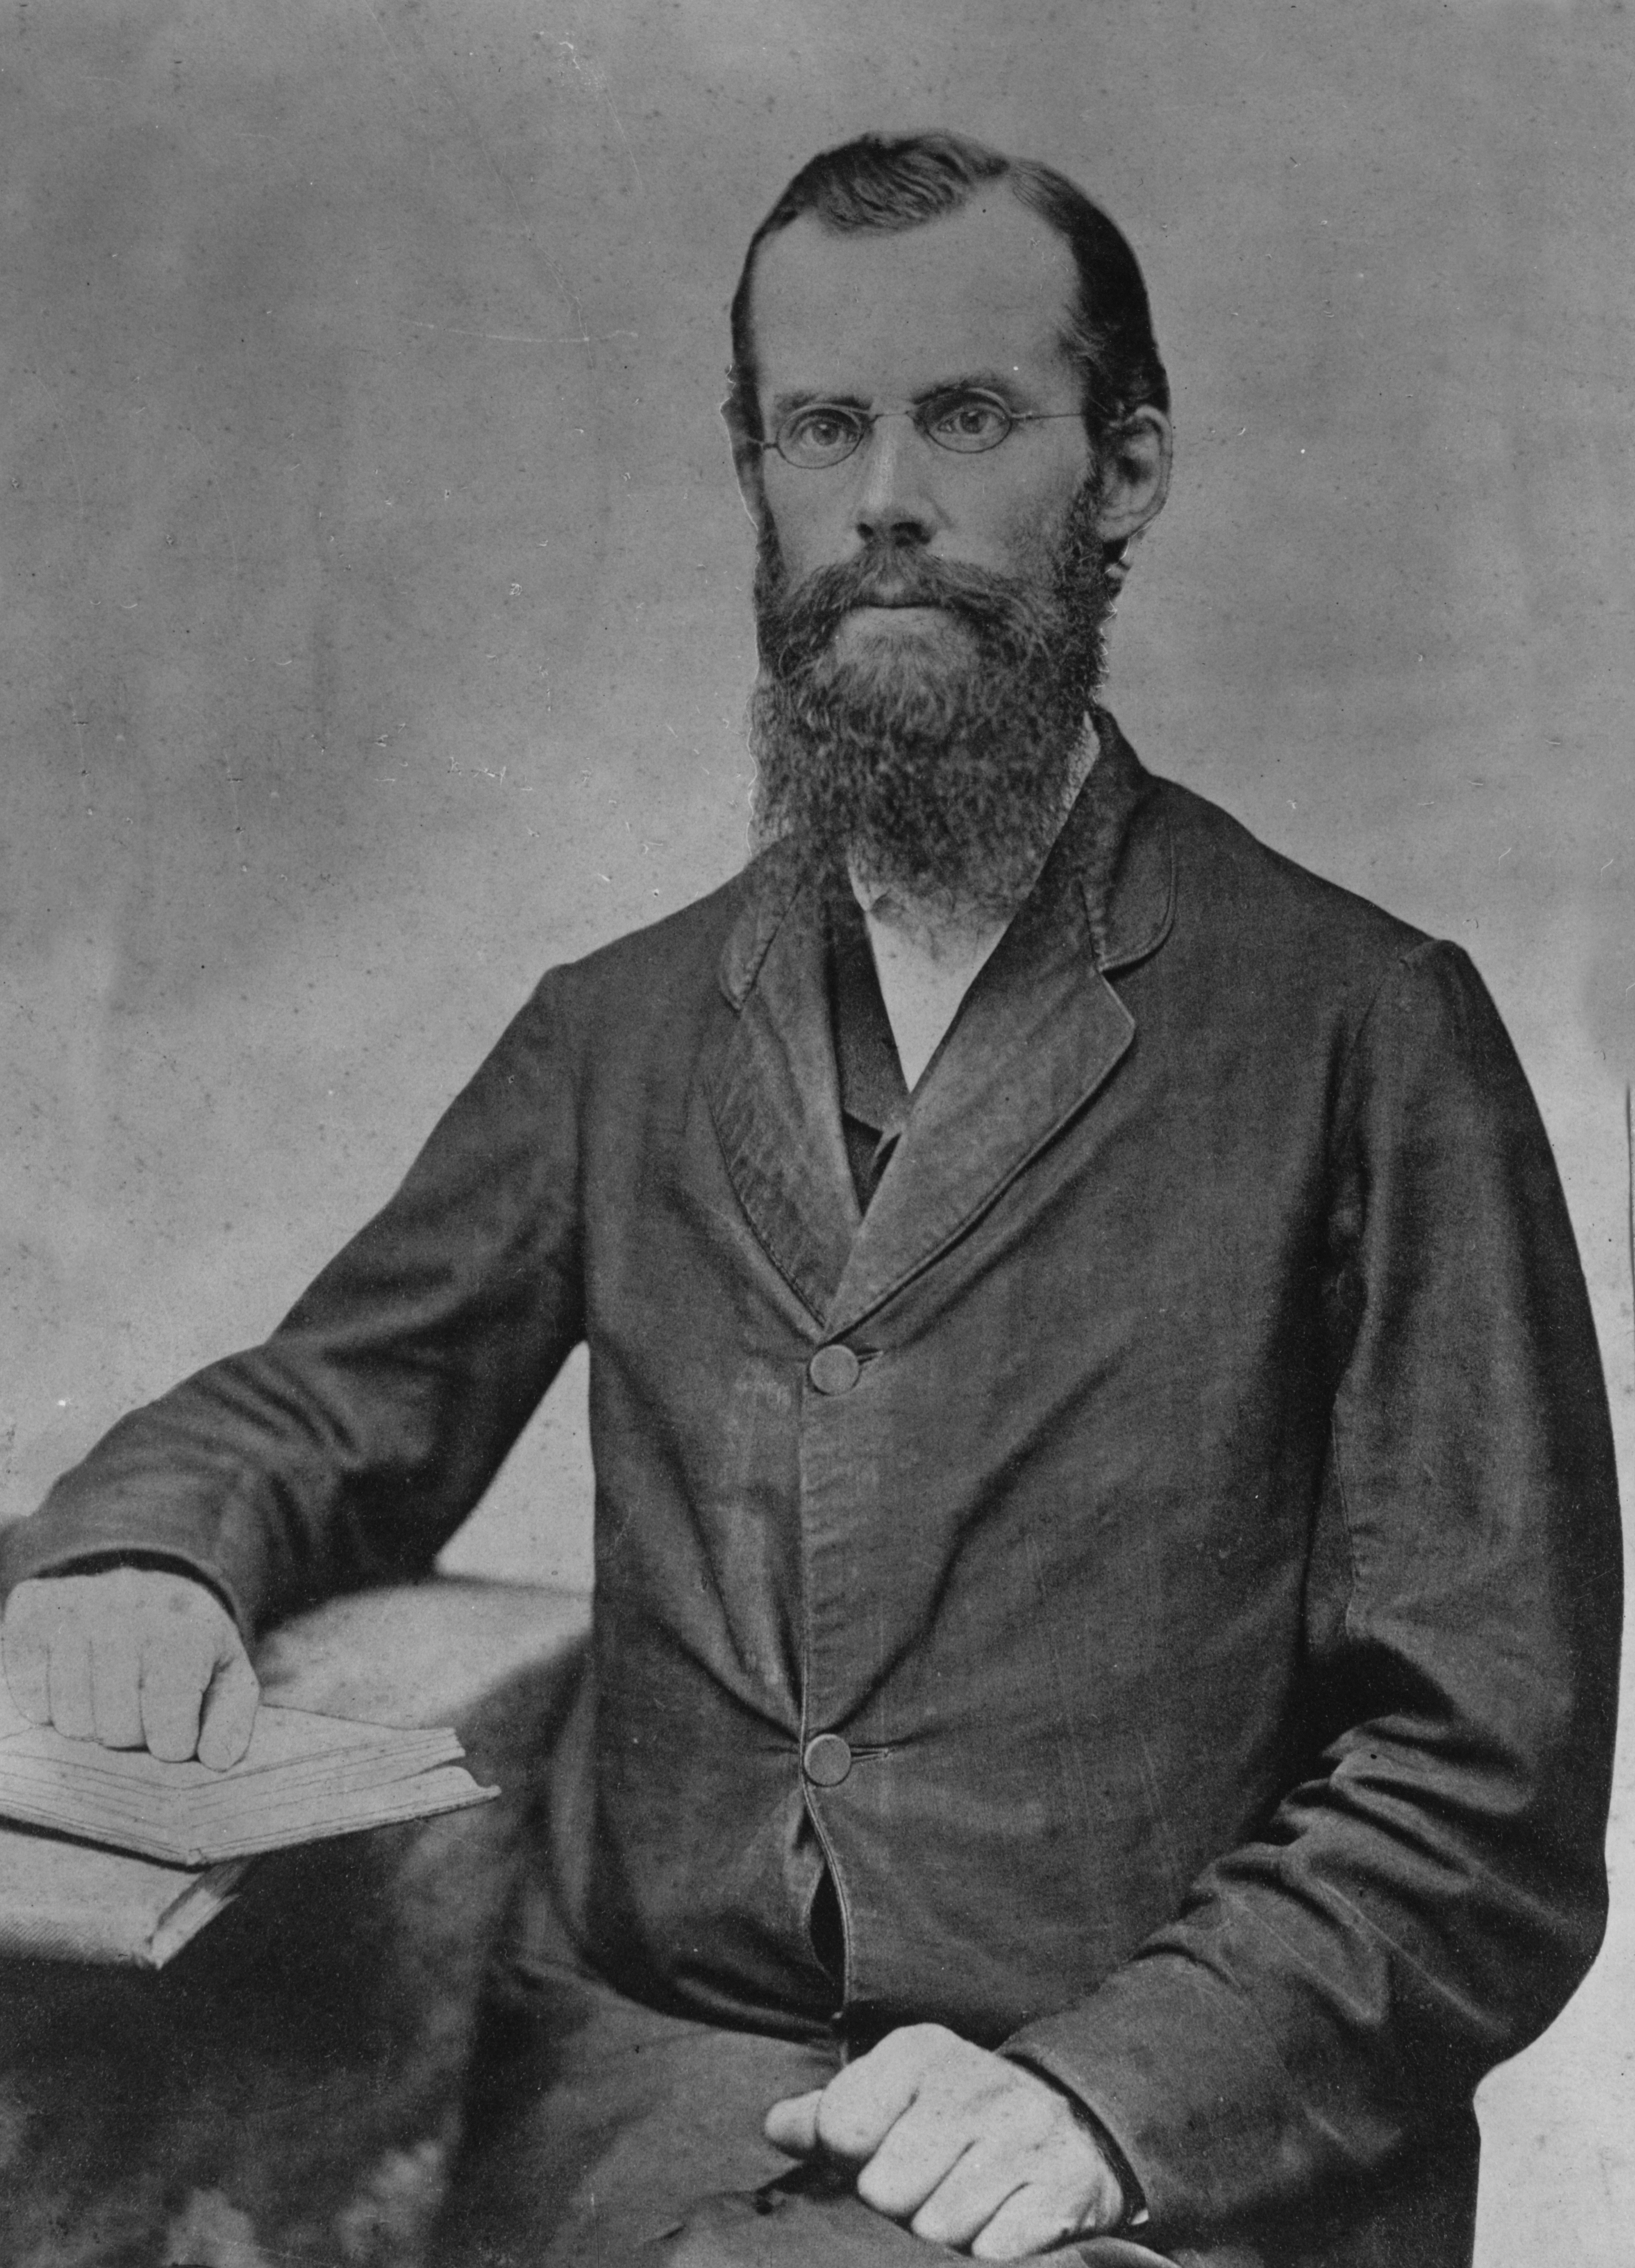
\includegraphics[width=1\linewidth]{images/john-nevins-andrews.jpg}
    \caption*{John Nevins Andrews (1829-1883)}
    \label{fig:j-n-andrews}
\end{figure}

J. N. Andrews alisema, \others{\textbf{Fundisho la Utatu ambalo lilianzishwa katika kanisa na Baraza la Nicea, A. D. 325}. \textbf{Fundisho hili \underline{linaharibu Umbile la Mungu, na Mwanawe Yesu Kristo Bwana wetu}}...}[John. N. Andrews, The Advent Review and Sabbath Herald, March 6, 1855, p. 185][http://documents.adventistarchives.org/Periodicals/RH/RH18550306-V06-24.pdf]

Katika muktadha wa ufahamu wa utatu kuhusu Umbile la Mungu, ni salama kusema kwamba Umbile la Mungu, au Ubora au hali ya Mungu kuwa Nafsi, katika ufahamu wowote ule wa Fundisho la Utatu ni swala lililo fumbo. Shida ni kwamba hakuna maoni wazi ya nani huyo \textit{Mungu mmoja} ambaye ni nafsi? Dai la msingi linafanywa kwamba Mungu ni Mmoja bado ni Watatu, au Mmoja ndani Tatu; ndio, Mungu ni Nafsi, na Yeye ni mmoja, lakini wakati huo huo Yeye ni nafsi tatu. Hii mtazamo hauwezi kamwe kushikilia mtazamo wowote wazi wa Umbile la Mungu. Pia, itakataa ushuhuda wa wazi kabisa wa Maandiko kwamba Mungu mmoja ndiye Baba, na kwamba Kristo ndiye kweli Mwana wake mzaliwa wa pekee. Ndugu wengi wa utatu wangekubali kwamba Kristo ni halisi na wa uhakika lakini ikiwa mwamini-utatu angemkubali Baba kama Huluki halisi na dhahiri, angemkubali pia Roho Mtakatifu kama Huluki halisi na dhahiri, hivyo kumkana Roho Mtakatifu kama kuwa \textit{roho}, njia ambayo kwayo Baba na Mwana wako kila mahali. Kinyume chake, ikiwa wa utatu wangemkubali Roho Mtakatifu kuwa Roho halisi, asiye na mwili wala umbo, basi yeye angemkana Baba kuwa Huluki halisi na dhahiri. Katika mazungumzo juu ya Ubora au hali ya Mungu kuwa Nafsi, hakuna kamwe maoni wazi ya jambo hilo kutoka kwa waendelezaji wa mafundisho ya Utatu; ni hila. \textit{‘Hila’} ni neno ambalo Dada White alitumia kuelezea udanganyifu huo wa usanii au ili kuficha, kuepuka, au kukwepa\footnote{\href{https://www.merriam-webster.com/dictionary/subterfuges}{The Merriam-Webster, ‘subterfuges’} - “\textit{deception by artifice or stratagem in order to conceal, escape, or evade}”} ukweli; kwa maneno mengine, kitu ambacho huwezi kunyakua kwa kichwa au mkia. Hii ndiyo sababu kuu ya Dada White kufanya kutojihusisha na majadiliano ya Utatu ambayo yangetokea katika kanisa la Waadventista Wasabato.

\egw{Nilitahadharishwa nisiingie kwenye mabishano \textbf{kuhusiana na swali} litakalo\textbf{\underline{jitokeza}} juu ya \textbf{mambo haya, kwa sababu mabishano yanaweza \underline{kusababisha watu kutumia hila, na akili zao zingeongozwa mbali na kweli wa Neno la Mungu hadi kwenye dhana na kazi ya kubahatisha}}. \textbf{Kadiri nadharia potofu zinavyojadiliwa, \underline{ndivyo wanadamu watakavyojua kidogo kuhusu Mungu na wa ile kweli inayotakasa nafsi}}.}[Lt232-1903.41; 1903][https://egwwritings.org/read?panels=p10197.50]

Tunaposoma kazi za waanzilishi wa Waadventista Wasabato juu ya Umbile la Mungu, tunaona kwamba hawakuanguka katika mtego wa Utatu. Maoni yao yasiyo ya utatu juu ya Mungu hayakukwa juu ya kutokwa na hekima, bali ujuzi wa ukweli juu ya Umbile la Mungu. Walikuwa na nia na akili nzuri, kuelewa mstari mwembamba kati ya ukweli na makosa. Uelewa wao wa Umbile la Mungu umelingana na kutoshana na kipimio, inaungwa mkono kwa nguvu kwa tamko lililo rahisi na wazi “\textit{Bwana asema hivi}”.

Waadventista wengi leo wanakubali fundisho la Utatu kwa sababu Ellen White kwa madhanio ya watu, alikuja kuikubali na kuikuza. Hii ni mbali na ukweli na hitimisho kama hilo linatabiriwa kukosa ujuzi wa Roho ya Unabii. Ikiwa mtu yeyote alikuwa anafahamu imani za Dada White, alikuwa mume wake James White. Hapa kuna anachosema juu ya maandishi ya mkewe:

\others{\textbf{Tunawaalika wote kulinganisha shuhuda za Roho Mtakatifu kupitia Bi. W., na neno la Mungu}. \textbf{Na katika hili hatukualiki kulinganisha \underline{na itikadi yako}}. Hiyo ni jambo jingine kabisa. \textbf{\underline{Mwenye kuamini utatu anaweza kuzilinganisha na imani yake, na kwa sababu hazikubaliani nayo, wanatoa hukumu}}. Anayeomba Jumapili, au mtu anayeshikilia mateso ya milele kama ukweli muhimu, na mtumishi anayenyunyizia watoto wachanga kwa ubatizo, wanaweza kila mmoja wao kulaani shuhuda’ za Bi. W. kwa sababu hazikubaliani na maoni yao ya kipekee. Na mia zaidi, kila mmoja akiwa na maoni tofauti, anaweza kufikia mkataa uleule. \textbf{Lakini uhalisi wao kamwe hauwezi kujaribiwa kwa namna hii}.}[James S. White, The Advent Review, and Herald of the Sabbath, June 13, 1871][https://documents.adventistarchives.org/Periodicals/RH/RH18710613-V37-26.pdf]

James White alikuwa mshirika wa karibu zaidi wa Ellen White, mtu ambaye alikuwa mmoja naye katika kuliinua Kanisa la Waadventista Wasabato. Tuna ushuhuda wa wazi na wa moja kwa moja kutoka kwake kwamba maandishi ya Ellen White si ya utatu. Leo, wasomi huweka hadithi za uwongo kwamba Ellen White alikua katika ufahamu wake wa fundisho la Utatu, na hatimaye akakubali na kuihubiri. Lakini tunaona kwamba Ellen White hakubadilisha maoni yake juu ya Umbile la Mungu wala hakushikamana na fundisho la Utatu. Alikuwa wazi kwa kudai kwamba hakuwahi kufanya hivyo. Wakati mzozo wa Kellogg ulipokuja juu ya Umbile la Mungu, yeye alibaki imara katika maoni yake, kama vile mapainia wote wa mapema wa Waadventista Wasabato walivyofanya—na mahusiano yake na Dk. Kellogg yanathibitisha hilo. Ni kweli, fundisho la Utatu \textit{haliwezi kukubaliwa na wale ambao ni waaminifu kwa imani na kwa kanuni ambazo zimestahimili upinzani wote wa ushawishi wa kishetani}.\footnote{\egw{Nadharia za Kiraka haziwezi kukubaliwa na wale ambao ni waaminifu kwa imani na kwa kanuni ambazo zimestahimili upinzani wote wa ushawishi wa kishetani}[Lt253-1903.28; 1903][https://egwwritings.org/read?panels=p14068.9980036]} Simulizi rasmi ya leo kwamba Ellen White alikuwa akifundisha Utatu inaangazia madai ya Dk. Kellogg kwamba The Living Temple ilifundisha kitu sawa na Ellen White. \egwinline{\textbf{Lakini Mwenyezi Mungu apishe mbali hisia hii kuwa na nguvu}.}[SpTB02 53.3; 1904][https://egwwritings.org/read?panels=p417.272]

% Adventist pioneers and the Trinity doctrine

\begin{titledpoem}
    \stanza{
        The pioneers stood firm against the Trinity's sway, \\
        Their testimony clear as the light of day. \\
        They saw how this doctrine did subtly disguise, \\
        What Scripture reveals to discerning eyes.
    }

    \stanza{
        James White declared it among "popular fables" found, \\
        A teaching that makes God's personality unsound. \\
        For Father and Son as distinct beings stand, \\
        Not merged into one as the Trinity planned.
    }

    \stanza{
        Two separate persons with purpose aligned, \\
        In spirit and action, united in mind. \\
        Just as disciples in Christ become one, \\
        Yet remain individual under God's Son.
    }

    \stanza{
        The Holy Spirit, God's presence divine, \\
        Not a separate being of the Godhead's design. \\
        But truly God's Spirit sent forth from above, \\
        The Father's representative, agent of love.
    }

    \stanza{
        No Scripture supports what tradition declared, \\
        When at Nicea this doctrine was shared. \\
        John seventeen shatters the trinitarian view, \\
        Revealing the Father and Son as beings true.
    }

    \stanza{
        Christ's divinity rests not in mysterious three, \\
        But in His begotten Sonship we see. \\
        The express image of His Father's face, \\
        Inheriting fullness of divine grace.
    }

    \stanza{
        The pioneers knew what the Bible made clear, \\
        That God is the Father, a Being most dear. \\
        A personal, spiritual presence on high, \\
        Omnipresent through Spirit, yet dwelling on high.
    }

    \stanza{
        So stands the truth against error's long night, \\
        Preserved by the pioneers and Sister White. \\
        Not through confusion or mystical thought, \\
        But through plain Scripture the truth has been taught.
    }
\end{titledpoem}
